\documentclass[tikz,border=8pt]{standalone}
% Shared look for every TikZ diagram. Load with \input{../../tools/tikz-style.tex}
\usepackage[T1]{fontenc}
\usepackage{lmodern}
\renewcommand{\sfdefault}{lmr}  % diagrams use the same serif as the text
\usetikzlibrary{arrows.meta, positioning, shapes.geometric, calc, fit, backgrounds}
\definecolor{cblue}{HTML}{4C78A8}
\definecolor{corange}{HTML}{F58518}
\definecolor{cgreen}{HTML}{54A24B}
\definecolor{cred}{HTML}{E45756}
\definecolor{cpurple}{HTML}{B279A2}
\definecolor{cgrey}{HTML}{6B6B6B}
\tikzset{
  every picture/.style={font=\sffamily, line width=1.2pt},
  box/.style={draw=#1, fill=#1!12, rounded corners=4pt, align=center, inner sep=7pt, minimum height=1.1cm},
  box/.default=cgrey,
  arrow/.style={-{Stealth[length=3mm]}, draw=cgrey, line width=1.4pt},
  title/.style={font=\sffamily\bfseries\Large},
  note/.style={font=\sffamily\small, text=cgrey, align=center},
}
\AtBeginDocument{\hyphenpenalty=10000 \exhyphenpenalty=10000}

\begin{document}
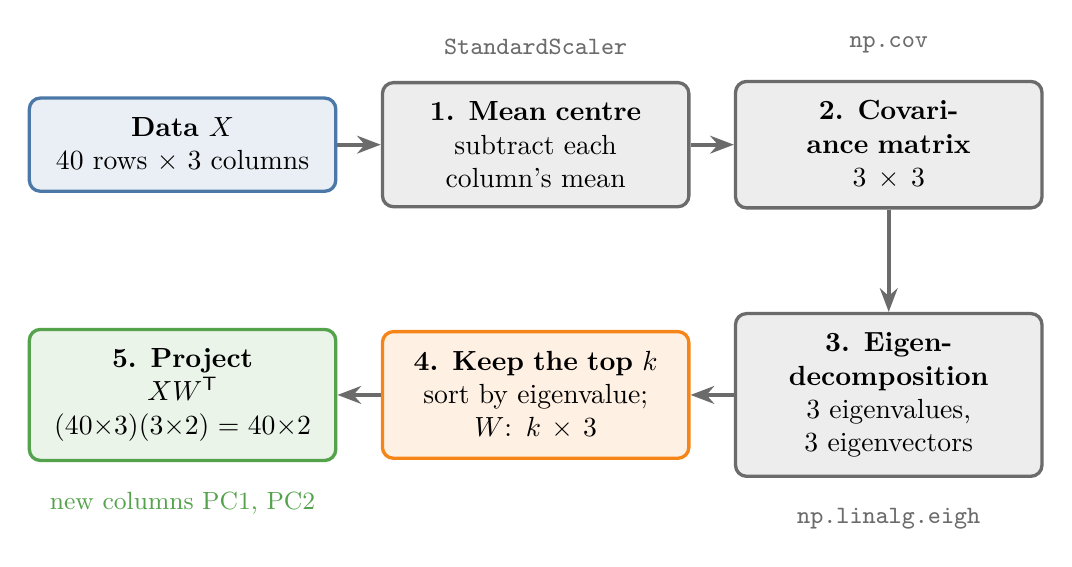
\begin{tikzpicture}[node distance=0.55cm]
  \node[box=cblue, text width=3.4cm] (d) {\textbf{Data} $X$\\40 rows $\times$ 3 columns};
  \node[box=cgrey, text width=3.4cm, right=of d] (s1) {\textbf{1. Mean centre}\\subtract each column's mean};
  \node[box=cgrey, text width=3.4cm, right=of s1] (s2) {\textbf{2. Covariance matrix}\\$3 \times 3$};
  \node[box=cgrey, text width=3.4cm, below=1.3cm of s2] (s3) {\textbf{3. Eigen-}\\\textbf{decomposition}\\3 eigenvalues,\\3 eigenvectors};
  \node[box=corange, text width=3.4cm, left=of s3] (s4) {\textbf{4. Keep the top $k$}\\sort by eigenvalue;\\$W$: $k \times 3$};
  \node[box=cgreen, text width=3.4cm, left=of s4] (s5) {\textbf{5. Project}\\$X W^{\mathsf T}$\\$(40{\times}3)(3{\times}2) = 40{\times}2$};
  \draw[arrow] (d) -- (s1); \draw[arrow] (s1) -- (s2); \draw[arrow] (s2) -- (s3);
  \draw[arrow] (s3) -- (s4); \draw[arrow] (s4) -- (s5);
  \node[note, below=0.25cm of s3] {\texttt{np.linalg.eigh}};
  \node[note, above=0.2cm of s2] {\texttt{np.cov}};
  \node[note, above=0.2cm of s1] {\texttt{StandardScaler}};
  \node[note, below=0.25cm of s5, text=cgreen] {new columns PC1, PC2};
\end{tikzpicture}
\end{document}
